%%%%%%%%%%%%%%%%%%%%%%%%%%%%%%%%%%%%%%%%%%%%%%%%%%%%%%%%%%%%%%%%%%%%%%
% Lớp 10 | Xác suất | Không gian mẫu và biến cố
% Dạng 0D0?1-3: Đếm phần tử không gian mẫu, biến cố 
% Số câu: 50  (sinh tự động bởi tach_cau.py; từ nay thầy sửa trực tiếp file này)
%%%%%%%%%%%%%%%%%%%%%%%%%%%%%%%%%%%%%%%%%%%%%%%%%%%%%%%%%%%%%%%%%%%%%%

%%%%%%%%%%%%%%%% TRẮC NGHIỆM 4 PHƯƠNG ÁN %%%%%%%%%%%%%%%%

% nguồn: MaHoaNH_TracNghiem_Lop10
\begin{ex}%[0D0N1-3]%[ma:859b5bd4]
	 Gieo một đồng xu liên tiếp $2$ lần. Số phần tử của không gian mẫu bằng
	 \choice
		 {\True $4$}
		 {$8$}
		 {$1$}
		{$2$} 
	\loigiai{Số phần tử của không gian mẫu $n  \left(\Omega\right)=\mathrm{C}_2^1\cdot \mathrm{C}_2^1=4$.
	} 
\end{ex}

% nguồn: MaHoaNH_TracNghiem_Lop10
\begin{ex}%[0D0N1-3]%[ma:3f7a659c]
	Một nhóm có $3$ bạn nam và $2$ bạn nữ. Chọn ngẫu nhiên cùng lúc $2$ bạn đi làm vệ sinh lớp. Số phần tử của không gian mẫu của phép thử  là
	 \choice
		 {\True $10$}
		{$5$} 
		{$15$} 
		{$2$} 
	 \loigiai{
		Do ta chọn $2$ bạn khác nhau từ $5$ bạn trong nhóm và không tính thứ tự nên số phần tử của không gian mẫu là $n\left(\Omega\right) = \mathrm{C}_{5}^{2}  = 10$.\\
	} 
\end{ex}

% nguồn: MaHoaNH_TracNghiem_Lop10
\begin{ex}%[0D0N1-3]%[ma:c66cdbaf]
	Gieo ngẫu nhiên  một đồng tiền cân đối và đồng chất $5$ lần. Tính số phần tử của không gian mẫu $\Omega$.
	 \choice
		 {$n(\Omega)=5$}
		 {\True $n(\Omega)=32$}
		 {$n(\Omega)=10$}
		{$n(\Omega)=120$} 
	\loigiai{ 
		Mỗi lần gieo đồng tiền, ta có  thể nhận được $2$ kết quả khác nhau, do đó khi gieo đồng tiền $5$ lần, số phần tử của không gian mẫu là $n(\Omega)=2^5=32$.
	 }
\end{ex}

% nguồn: MaHoaNH_TracNghiem_Lop10
\begin{ex}%[0D0N1-3]%[ma:bc69da88]
	Tung một đồng xu cân đối và đồng  chất hai lần. Số phần tử của biến cố cả hai lần tung đều xuất hiện mặt sấp là
	 \choice
		 {\True $1$}
		 {$3$}
		 {$2$}
		 {$4$}
	 \loigiai{
		Số phần tử của biến cố cả hai  lần tung đều xuất hiện mặt sấp là $1$.
	 }
\end{ex}

% nguồn: MaHoaNH_TracNghiem_Lop10
\begin{ex}%[0D0N1-3]%[ma:a56fe366]
	Gieo một con súc sắc. Số phần tử  của không gian mẫu là?
	\choice 
		 {$24$}
		 {$12$}
		 {$8$}
		{\True  $6$}
	\loigiai{ 
		Vì một con  súc sắc có $6$ mặt có số nút mỗi mặt khác nhau nên số phần tử của không gian mẫu trong phép thử gieo một súc sắc là $6$.
	 }
\end{ex}

% nguồn: MaHoaNH_TracNghiem_Lop10
\begin{ex}%[0D0N1-3]%[ma:16680692]
	Một con xúc sắc cân đối đồng chất có $6$ mặt được viết các số $3$; $4$; $5$; $6$; $7$; $8$ trên mỗi mặt. Xét phép thử ngẫu nhiên gieo xúc sắc một lần. Tính số phần tử của không gian  mẫu.
	 \choice
		{$5$} 
		 {\True $6$}
		 {$8$}
		{$3$} 
	 \loigiai{
		Không  gian mẫu là $\Omega=\{3;4;5;6;7;8\}$.\\
		Vậy  không gian mẫu gồm $6$ phần tử.
	 }
\end{ex}

% nguồn: MaHoaNH_TracNghiem_Lop10
\begin{ex}%[0D0H1-3]%[ma:c5b00e2e]
	Một hộp  đựng $10$ sản phẩm tốt và $3$ sản phẩm kém chất lượng, rút ngẫu nhiên từ trong hộp ra $3$ sản phẩm. Số phần tử của không gian mẫu là
	 \choice
		 {$\mathrm{C}_{10}^3$}
		 {$\mathrm{C}_3^3$}
		 {$\mathrm{C}_7^3$}
		 {\True $\mathrm{C}_{13}^3$}
	\loigiai{Số phần tử không gian mẫu là là số cách chọn  $3$ sản phẩm từ $13$ sản phẩm đã cho nên số phần tử không gian mẫu là $n(\Omega)=\mathrm{C}_{13}^3$.}
\end{ex}

% nguồn: MaHoaNH_TracNghiem_Lop10
\begin{ex}%[0D0H1-3]%[ma:6de7881c]
	Rút ngẫu nhiên cùng lúc ba con bài từ cỗ  bài tú lơ khơ $52$ con thì $n(\Omega)$ bằng bao nhiêu?
	\choice 
		{$140\,608$} 
		{$156$} 
		 {$132\,600$}
		{\True $22\,100$} 
	\loigiai{Ta  có $n(\Omega)=\mathrm{C}_{52}^3=22\,100$.}
\end{ex}

% nguồn: MaHoaNH_TracNghiem_Lop10
\begin{ex}%[0D0H1-3]%[ma:811cd64d]
	Gieo một đồng tiền liên tiếp $2$ lần. Số phần tử của không gian mẫu $n(\Omega)$ là 
	 \choice
		{$1$} 
		 {$2$}
		{\True  $4$}
		{$8$} 
	\loigiai{Số phần  tử của không gian mẫu $n(\Omega)=2\cdot 2=4$.
	 }
\end{ex}

% nguồn: MaHoaNH_TracNghiem_Lop10
\begin{ex}%[0D0H1-3]%[ma:4e6d42ec]
	Gieo ngẫu nhiên $2$ đồng tiền thì không gian mẫu của phép thử có bao  nhiêu phần tử?
	 \choice
		 {\True $4$}
		 {$8$}
		 {$12$}
		 {$16$}
	\loigiai{Mô tả không gian mẫu ta có $\Omega=\{SS;SN;NS;NN\}$. 
	 }
\end{ex}

% nguồn: MaHoaNH_TracNghiem_Lop10
\begin{ex}%[0D0H1-3]%[ma:787eb05f]
	Gieo đồng tiền hai lần. Số phần tử của biến cố để mặt ngửa xuất  hiện đúng $1$ lần là
	\choice 
		 {\True $2$}
		{$4$} 
		 {$5$}
		 {$6$}
	 \loigiai{Liệt kê ta có $A=\{NS;SN\}$.
	 }
\end{ex}

% nguồn: MaHoaNH_TracNghiem_Lop10
\begin{ex}%[0D0H1-3]%[ma:35dffa20]
	Gieo một con súc sắc $2$ lần. Số phần tử  của không gian mẫu là
	\choice 
		 {$6$}
		 {$12$}
		 {$18$}
		{\True $36$} 
	\loigiai{Số phần tử của không gian mẫu $n(\Omega)=6\cdot  6=36$.
	 }
\end{ex}

% nguồn: MaHoaNH_TracNghiem_Lop10
\begin{ex}%[0D0H1-3]%[ma:e8b8b991]
	Gieo một đồng tiền và một con súc sắc. Số  phần tử của không gian mẫu là
	 \choice
		 {$24$}
		{\True  $12$}
		{$6$} 
		 {$8$}
	\loigiai{Mô tả không gian mẫu ta có  $\Omega=\{S1;S2;S3;S4;S5;S6;N1;N2;N3;N4;N5;N6\}$.
	 }
\end{ex}

% nguồn: MaHoaNH_TracNghiem_Lop10
\begin{ex}%[0D0H1-3]%[ma:ea20cabf]
	Gieo một con súc sắc liên tiếp hai lần. Gọi $A$ là biến cố \lq\lq kết quả hai lần gieo như nhau\rq\rq. Tính số phần tử  của biến cố $A$.
	 \choice
		 {\True $n(A)=6$}
		 {$n(A)=12$}
		{$n(A)=1$} 
		{$n(A)=8$} 
	 \loigiai{
		 Ta có $A=\left\{(1;1),(2;2),(3;3),(4;4),(5;5),(6;6)\right\}\Rightarrow n(A)=6$.
	 }
\end{ex}

% nguồn: MaHoaNH_TracNghiem_Lop10
\begin{ex}%[0D0H1-3]%[ma:2c5f6eab]
	 Trong một chiếc hộp đựng $6$ viên bi đỏ, $8$ viên bi xanh, $10$ viên bi trắng. Lấy ngẫu nhiên $4$ viên bi. Số phần tử của không gian mẫu là
	\choice 
		{\True $n(\Omega) =  \mathrm{C}_{24}^{4}$}
		{$n(\Omega)  = \mathrm{A}_{24}^{4}$}
		{$n(\Omega) = \mathrm{C}_{6}^{4} + \mathrm{C}_{8}^{4} +  \mathrm{C}_{10}^{4}$}
		 {$n(\Omega) = 6\cdot 8\cdot 10$}
	\loigiai{ 
		 Số phần tử của không gian mẫu là $n(\Omega) = \mathrm{C}_{24}^{4}$.
	} 
\end{ex}

% nguồn: MaHoaNH_TracNghiem_Lop10
\begin{ex}%[0D0H1-3]%[ma:6eef9f7a]
	Có $100$ tấm thẻ được đánh số từ $1$ đến $100$. Lấy ngẫu nhiên $5$ thẻ. Số phần tử của không gian  mẫu là
	 \choice
		{\True $n(\Omega) =  \mathrm{C}_{100}^{5}$}
		{$n(\Omega) =  \mathrm{A}_{100}^{5}$}
		{$n(\Omega)  = \mathrm{C}_{100}^{1}$}
		{$n(\Omega) = \mathrm{A}_{100}^{1}$} 
	\loigiai{ 
		Số phần tử của  không gian mẫu là $n(\Omega) = \mathrm{C}_{100}^{5}$.
	} 
\end{ex}

% nguồn: MaHoaNH_TracNghiem_Lop10
\begin{ex}%[0D0H1-3]%[ma:c915dd6f]
	Gieo con xúc xắc hai lần. Gọi $ A $ là biến cố \lq\lq Sau hai lần gieo có ít nhất một mặt $ 3 $ chấm\rq\rq. Các kết quả thuận lợi cho  biến cố $ A $ là
	\choice 
		 {$ A=\left\lbrace (3;1),(3;2),(3;3),(3;4),(3;5),(3;6)\right\rbrace $}
		{$ A=\left\lbrace  (1;3),(2;3),(3;3),(4;3),(5;3),(6;3)\right\rbrace $}
		{$  A=\left\lbrace (3;1),(3;2),(3;4),(3;5),(3;6),(1;3),(2;3),(4;3),(5;3),(6;3)\right\rbrace $}
		{\True $ A=\left\lbrace (3;1),(3;2),(3;3),(3;4),(3;5),(3;6),(1;3),(2;3),(4;3),(5;3),(6;3)\right\rbrace $} 
	\loigiai{ 
		Các kết quả thuận lợi cho biến cố $ A  $ là $$ A=\left\lbrace (3;1),(3;2),(3;3),(3;4),(3;5),(3;6),(1;3),(2;3),(4;3),(5;3),(6;3)\right\rbrace. $$
	} 
\end{ex}

% nguồn: MaHoaNH_TracNghiem_Lop10
\begin{ex}%[0D0H1-3]%[ma:226500bf]
	Gieo một con xúc xắc cân đối và đồng chất hai lần. Số phần tử của không gian mẫu  là
	\choice 
		{\True  $36$}
		 {$12$}
		 {$6$}
		{$18$} 
	\loigiai{ 
		Số phần tử của không gian mẫu khi gieo một con xúc xắc cân đối đồng chất hai lần là  $36$.
	 }
\end{ex}

% nguồn: MaHoaNH_TracNghiem_Lop10
\begin{ex}%[0D0H1-3]%[ma:3bcee9b8]
	 Gieo ngẫu nhiên một con súc sắc hai lần. Xét biến cố $A$: \lq\lq Lần thứ hai xuất hiện mặt ba chấm\rq\rq\ thì biến cố $A$ là
	 \choice
		{$A=\{(3;1);(3;2);(3;3);(3;4);(3;5);(3;6)\}$} 
		{$A=\{(3;1);(3;2);(3;4);(3;5);(3;6)\}$} 
		{\True $A=\{(1;3);(2;3);(3;3);(4;3);(5;3);(6;3)\}$} 
		{$A=\{(3;3)\}$} 
	 \loigiai{
		Ký hiệu $(i;j)$ là số chấm xuất hiện lần  lượt ở lần một và lần hai khi gieo con súc sắc, trong đó $i,j\in\{1;2;3;4;5;6\}$.\\
		Xét biến cố $A$: \lq\lq Lần thứ hai xuất hiện mặt ba chấm\rq\rq\ thì $j=3$ còn $i$ là một số tự nhiên bất  kỳ trong phạm vi từ $1$ đến $6$.
	 }
\end{ex}

% nguồn: MaHoaNH_TracNghiem_Lop10
\begin{ex}%[0D0H1-3]%[ma:ef36b253]
	Số phần tử của không gian mẫu trong phép thử  $T$: \lq\lq Tung một con xúc xắc cân đối và đồng chất $2$ lần\rq\rq\, là
	\choice 
		{$3$} 
		{$64$} 
		{\True  $36$}
		 {$12$}
	\loigiai{ 
		Ta có $\Omega=\{(i,j)\mid i=1,2,\ldots,6;  j=1,2,\ldots,6\}$.\\
		Do đó $n(\Omega)=6\cdot 6=36$. 
	} 
\end{ex}

% nguồn: MaHoaNH_TracNghiem_Lop10
\begin{ex}%[0D0H1-3]%[ma:27f9fcbd]
	Một nhóm gồm $6$ học sinh nam và $4$ học sinh nữ. Chọn ngẫu nhiên cùng lúc 5học sinh để tham gia công tác tình nguyện. Số  kết quả thuận lợi của biến cố $D$: \lq\lq $5$ học sinh được chọn có ít nhất $1$ học sinh nữ\rq\rq\ là
	 \choice
		 {$60$}
		{\True  $246$}
		{$186$} 
		 {$180$}
	 \loigiai{
		Số cách chọn $5$ học sinh bất kì từ $10$ học sinh  là $\mathrm{C}_{10}^5$.\\
		Số cách chọn  $5$ học sinh đều là học $\sinh$ nam là $\mathrm{C}_6^5$.\\
		Do đó số kết quả thuận lợi của biến cố  $D$ là $n(D)=\mathrm{C}_{10}^5-\mathrm{C}_6^5=246$.
	 }
\end{ex}

% nguồn: MaHoaNH_TracNghiem_Lop10
\begin{ex}%[0D0H1-3]%[ma:864061c6]
	Một  đội thanh niên tình nguyện gồm $12$ nam và $3$ nữ được phân công ngẫu nhiên về $3$ tỉnh, mỗi tỉnh $5$ người. Tính số phần tử của không gian mẫu.
	 \choice
		{$\mathrm{C}_{15}^5\cdot  \mathrm{C}_{14}^5\cdot \mathrm{C}_{13}^5$}
		{\True $\mathrm{C}_{15}^5\cdot \mathrm{C}_{10}^5\cdot \mathrm{C}_5^5$} 
		 {$\mathrm{C}_{15}^5$}
		{$\mathrm{C}_{12}^4\cdot  \mathrm{C}_3^1$}
	\loigiai{Chọn $5$ người từ $15$ người  về tỉnh thứ nhất có $\mathrm{C}_{15}^5$ cách.\\
		Chọn $5$ người từ $10$ người còn lại về tỉnh thứ hai có $\mathrm{C}_{10}^5$  cách.\\
		Chọn $5$ người từ $5$ người về tỉnh thứ  ba có $\mathrm{C}_5^5$ cách chọn.\\
		 Suy ra có $\mathrm{C}_{15}^5\cdot \mathrm{C}_{10}^5\cdot \mathrm{C}_5^5$ cách phân công 1$5$ người về $3$ tỉnh, mỗi tỉnh $5$ người.\\
	Vậy số phần tử của không gian mẫu là $\mathrm{C}_{15}^5\cdot \mathrm{C}_{10}^5\cdot \mathrm{C}_5^5$.} 
\end{ex}

% nguồn: MaHoaNH_TracNghiem_Lop10
\begin{ex}%[0D0H1-3]%[ma:989035b8]
	Gieo một con súc sắc cân đối và đồng chất hai lần. Tính  số phần tử của biến cố: \lq\lq Tổng số chấm của hai lần gieo không quá $5$\rq\rq.
	\choice 
		{\True  $10$}
		 {$8$}
		{$11$} 
		{$9$} 
	 \loigiai{
		Các  trường hợp thuận lợi để biến cố xảy ra là
		$$\{(1;1),(1;2),(2;1),(1;3),(3;1),(1;4),(4;1),(2;2),(2;3),(3;2)\}.$$ 
		 Vậy có $10$ phần tử.
	 }
\end{ex}

% nguồn: MaHoaNH_TracNghiem_Lop10
\begin{ex}%[0D0H1-3]%[ma:352433e3]
	Xét phép  thử gieo một con súc sắc cân đối và đồng chất $6$ mặt hai lần. Xét biến cố $A$: \lq\lq Số chấm xuất hiện ở cả hai lần gieo giống nhau\rq\rq. Khẳng định nào sau đây đúng?
	\choice 
		 {\True $n(A)=6$}
		{$n(A)=12$} 
		 {$n(A)=16$}
		{$n(A)=36$} 
	\loigiai{Gọi cặp số $(x;y)$ là số chấm xuất hiện ở hai lần  gieo.\\
		Xét biến cố $A$: \lq\lq Số chấm xuất hiện ở cả hai lần  gieo giống nhau\rq\rq.\\
		Các kết quả của biến cố $A$  là $\{(1;1);(2;2);(3;3);(4;4);(5;5);(6;6)\}$.\\
		Suy ra  $n(A)=6$.
	} 
\end{ex}

% nguồn: MaHoaNH_TracNghiem_Lop10
\begin{ex}%[0D0H1-3]%[ma:85bb8aa7]
	Từ các chữ số $1, 3, 5, 7, 9$ lập được bao nhiêu số  tự nhiên có $5$ chữ số khác nhau mà chữ số đầu tiên là chữ số $3$?
	 \choice
		{$4$ số} 
		 {$6$ số}
		{\True $24$ số} 
		{$12$ số} 
	 \loigiai{
		Số cần lập có dạng $\overline{abcde}$.\\ 
		Chữ số đầu tiên là chữ số $3$ nên $a=3$.\\ 
		Số cách lập $\overline{bcde}$ là $4!=24$.\\ 
		 Vậy lập được tất cả là $1\cdot 24=24$ số.
	} 
\end{ex}

% nguồn: MaHoaNH_TracNghiem_Lop10
\begin{ex}%[0D0H1-3]%[ma:126cce7a]
	Trong hộp có $15$ tấm thẻ được đánh số từ $1$ đến $15$. Lấy ngẫu nhiên từ trong hộp ra $2$ tấm thẻ. Số các kết  quả thuận lợi của biến cố \lq\lq Hai thẻ lấy ra có tổng là một số chẵn\rq\rq.
	\choice 
		{$35$} 
		{\True  $49$}
		 {$28$}
		{$21$} 
	\loigiai{ 
		Để hai thẻ lấy ra có tổng là một số chẵn thì hai thẻ đó là hai thẻ đều ghi  số lẻ hoặc ghi số chẵn.\\
		{\bfseries Trường hợp 1:}  Hai thẻ lấy ra đều ghi số lẻ có $\mathrm{C}_8^2=28$ cách.\\
		{\bfseries Trường  hợp 2:} Hai thẻ lấy ra đều ghi số chẵn có $\mathrm{C}_7^2=21$ cách.\\
		 Vậy có $28+21=49$ cách lấy ra hai thẻ lấy ra có tổng là một số chẵn.
	 }
\end{ex}

% nguồn: MaHoaNH_TracNghiem_Lop10
\begin{ex}%[0D0H1-3]%[ma:277813ef]
	Một hộp đựng bi gồm $5$ bi màu xanh và $6$ bi màu đỏ. Lấy 3 viên bi từ hộp. Có  bao nhiêu kết quả thuận lợi để có đúng $1$ bi màu xanh?
	\choice 
		 {$5$}
		 {$20$}
		 {$15$}
		 {\True $75$}
	\loigiai{Để  lấy được $ 3 $ bi \textbf{có đúng} $ 1 $ bi xanh ta thực hiện như sau:
	\begin{itemize}
		\item Lấy $1$ bi  màu xanh, số cách lấy là $\mathrm{C}^1_5=5$.
		\item Lấy tiếp thêm $ 2 $ bi màu đỏ, số  cách lấy là $\mathrm{C}^2_6=15$.
	\end{itemize}
	Vậy số kết quả  thuận lợi lấy $1$ bi màu xanh và $2$ bi màu đỏ là $5 \cdot 15 = 75$.
	 }
\end{ex}

% nguồn: MaHoaNH_TracNghiem_Lop10
\begin{ex}%[0D0H1-3]%[ma:8a1efde4]
	Từ một hộp chứa $16$ quả cầu gồm $7$ quả màu đỏ và $9$ quả màu xanh, lấy ngẫu nhiên đồng thời hai quả. Số kết quả  thuận lợi để lấy được hai quả có màu khác nhau bằng
	 \choice
		{$57$} 
		{\True $63$} 
		{$120$} 
		{$55$} 
	\loigiai{ 
		Lấy ngẫu nhiên đồng thời  hai quả cầu trong 16 quả cầu ta có $\mathrm{C}_{16}^2$ cách.\\
		Vậy số phần tử của không gian mẫu là $n(\Omega)=\mathrm{C}_{16}^2  = 120$.\\
		Gọi biến cố $A$ là \lq\lq lấy được hai quả có  màu khác nhau\rq\rq.\\
		Số cách chọn $2$ quả cầu chọn ra cùng màu  là $\mathrm{C}_5^3 + \mathrm{C}_6^3$, suy ra $n(\mathrm{\overline{A}})=\mathrm{C}_7^2 + \mathrm{C}_9^2 = 57$.\\
		Vì vậy $n\left(A\right) = n\left(\Omega\right)  - n\left(\overline{A}\right) = 120 - 57 = 63$.
	} 
\end{ex}

% nguồn: MaHoaNH_TracNghiem_Lop10
\begin{ex}%[0D0H1-3]%[ma:80f1d3b8]
	Một hộp chứa $11$ quả cầu gồm $5$ quả cầu màu xanh và $6$ quả cầu màu đỏ. Chọn ngẫu nhiên đồng thời $3$ quả cầu từ hộp đó. Số kết quả thuận lợi để $3$ quả cầu chọn ra không cùng màu là 
	\choice 
		{$153$} 
		{$165$} 
		{\True  $135$}
		{$156$} 
	\loigiai{ 
		Để  lấy $3$ trái cầu từ hộp ta có $\mathrm{C}_{11}^3$ cách.\\
		 Vậy số phần tử của không gian mẫu là $n(\Omega)=\mathrm{C}_{11}^3 = 165$.\\
		Đặt biến cố $\mathrm{A}$: \lq\lq $3$ quả cầu  chọn ra không cùng màu\rq\rq.\\
		Biến cố đối $\mathrm{\overline{A}}$: \lq\lq $3$  quả cầu chọn ra cùng màu\rq\rq.\\
		Số cách chọn  $3$ quả cầu chọn ra cùng màu là $\mathrm{C}_5^3 + \mathrm{C}_6^3$, suy ra $n(\mathrm{\overline{A}})=\mathrm{C}_5^3 + \mathrm{C}_6^3 = 30$.\\
		Vì vậy $n\left(A\right) = n\left(\Omega\right) - n\left(\overline{A}\right)  = 165 - 30 = 135$.
	} 
\end{ex}

% nguồn: MaHoaNH_TracNghiem_Lop10
\begin{ex}%[0D0H1-3]%[ma:e0467f61]
	Lớp $10A$ có $40$ học sinh với $16$ nữ và $24$ nam. Giáo viên chủ nhiệm cần chọn ra $4$  học sinh. Số phần tử của biến cố $A \colon$ \lq \lq trong số $4$ học sinh được chọn có ít nhất $2$ nữ\rq \rq \ là
	\choice 
		{\True $46560$} 
		 {$33120$}
		 {$48830$}
		 {$48756$}
	\loigiai{ 
		Gọi $A$ là biến cố \lq \lq trong số $4$ học  sinh được chọn có ít nhất $2$ nữ\rq \rq.
		\begin{itemize}
			\item Trường hợp $2$ nữ trong $4$ học sinh được chọn có $\mathrm{C}_{16}^2  \cdot \mathrm{C}_{24}^2$ cách.
			\item Trường hợp $3$ nữ trong $4$ học sinh được chọn  có $\mathrm{C}_{16}^3 \cdot \mathrm{C}_{24}^1$ cách.
		\end{itemize}
		Theo quy tắc cộng vậy ta có $n(A)=\mathrm{C}_{16}^2 \cdot \mathrm{C}_{24}^2+\mathrm{C}_{16}^3 \cdot  \mathrm{C}_{24}^1=46560$ cách.
	} 
\end{ex}

% nguồn: MaHoaNH_TracNghiem_Lop10
\begin{ex}%[0D0V1-3]%[ma:d23d4ec3]
	Cho tập hợp $A=\{0;1;2;3;4;5\}$, gọi $S$ là tập hợp các số có $3$ chữ số khác nhau được lập từ tập $A$. Chọn ngẫu nhiêu từ tập $S$ hai số bất kỳ, số các kết quả thuận lợi của biến cố \lq\lq Hai số được chọn đều là  số chia hết cho $5$\rq\rq\ là
	\choice 
		{$40$} 
		{$1260$} 
		 {$36$}
		{\True $630$} 
	 \loigiai{
		Gọi số có $3$ chữ số khác được lập từ  tập $A$ và chia hết cho $5$ có dạng $\overline{abc}$.\\
		{\bfseries Trường hợp 1:} Với  $c=0$ thì số cách lập được các số dạng này là $1\cdot A_5^2=20$ số.\\
		{\bfseries Trường hợp  2:} Với $c\neq0$ thì số cách lập được các số dạng này là $1\cdot 4\cdot 4=16$ số.\\
		Do đó, có $20+16=36$ số có $3$ chữ số phân biệt được lập từ tập $A$ chia  hết cho $5$.\\
		 Vậy số cách chọn ra hai số đều là số chia hết cho $5$ từ tập này là $\mathrm{C}_{36}^2=630$ cách.
	} 
\end{ex}

% nguồn: MaHoaNH_TracNghiem_Lop10
\begin{ex}%[0D0V1-3]%[ma:4771452e]
	Có hai dãy ghế đối diện nhau, mỗi dãy có $3$ ghế. Xếp ngẫu nhiên $6$ học sinh, gồm $3$ nam và $3$ nữ, ngồi vào hai dãy ghế đó sao cho mỗi ghế có đúng một học sinh ngồi. Số phần tử của biến cố \lq\lq các bạn học sinh nam ngồi đối  diện các bạn nữ \rq\rq\ là
	\choice 
		 {$144$}
		{$\dfrac{1}{20}$} 
		{\True $288$} 
		{$48$} 
	\loigiai{Gọi $A$ là biến cố: \lq\lq Các bạn học  sinh nam ngồi đối diện các bạn nữ\rq\rq.\\
		Chọn chỗ cho  học sinh nam thứ nhất có $6$ cách.\\
		Chọn chỗ cho học sinh nam thứ $2$ có $4$ cách (không ngồi đối diện học sinh nam thứ nhất).\\ 
		Chọn chỗ cho học sinh nam thứ  $3$ có $2$ cách (không ngồi đối diện học sinh nam thứ nhất, thứ hai).\\
		Xếp chỗ cho $3$ học sinh  nữ có $3!$ cách.\\
		Theo quy tắc nhân ta có $n(A)=6\cdot  4\cdot 2\cdot 3!=288$ cách.
	} 
\end{ex}

% nguồn: MaHoaNH_TracNghiem_Lop10
\begin{ex}%[0D0V1-3]%[ma:6163db2c]
	Chia ngẫu nhiên $25$ quyển vở giống nhau thành $4$ phần quà (phần nào cũng có vở). Tính số các kết quả thuận lợi của biến cố \lq\lq Mỗi phần quà  đều có ít nhất $4$ quyển vở\rq\rq.
	 \choice
		 {$56$}
		 {$336$}
		{\True $220$} 
		 {$1\,320$}
	 \loigiai{
		Để chia thành $4$ phần quà  mà mỗi phần có ít nhất $4$ quyển vở ta làm như sau:
		Chia mỗi phần là $3$ quyển vở. Còn lại $13$  quyển vở.\\
		Khi đó bài toán trở thành:  Có bao nhiêu cách chia $13$ quyển vở thành $4$ phần quà sao cho mỗi phần có ít nhất $1$ quyển vở.\\
		Để làm bài toán này ta xếp $13$ quyển vở thành hàng ngang, khi đó có $12$ khoảng trống  giữa các quyển vở.\\
		 Vậy có $\mathrm{C}_{12}^3=220$ cách chia.
	 }
\end{ex}

% nguồn: MaHoaNH_TracNghiem_Lop10
\begin{ex}%[0D0V1-3]%[ma:61610aba]
	Trong một chiếc hộp đựng $6$ viên bi đỏ, $8$ viên bi xanh, $10$ viên bi trắng. Lấy ngẫu nhiên $4$  viên bi. Tính số kết quả thuận lợi của biến cố $E$: \lq\lq $4$ viên bi lấy ra chỉ có $2$ màu\rq\rq.
	\choice 
		 {$916$}
		 {$4\,375$}
		{$2\,780$} 
		{\True  $5\,291$}
	\loigiai{Ta xét các trường hợp sau thuận lợi cho  biến cố $E$.\\
		{\bfseries Trường hợp 1:} Có $2$ màu đỏ  và xanh.\\
		Số cách lấy $4$ viên bi từ $14$ viên bi đỏ và xanh là $\mathrm{C}_{14}^4$, trong đó có $\mathrm{C}_6^4$ cách lấy chỉ có bi đỏ và $\mathrm{C}_8^4$ cách lấy chỉ có bi xanh. Do đó số cách lấy $4$ viên có đủ  hai màu xanh đỏ là $\mathrm{C}_{14}^4-\mathrm{C}_6^4-\mathrm{C}_8^4=916$ (cách).\\
		Tương tự ta có các trường hợp  sau đây.\\
		{\bfseries Trường hợp 2:} Có $2$ màu đỏ và trắng:  $\mathrm{C}_{16}^4-\mathrm{C}_6^4-\mathrm{C}_{10}^4=1\,595$ (cách).\\
		{\bfseries Trường hợp 3:} Có $2$ màu xanh và trắng: $\mathrm{C}_{18}^4-\mathrm{C}_8^4-\mathrm{C}_{10}^4=2\,780$  (cách).
		Vậy số kết quả thuận lợi của biến  cố $E$ là $n(E)=916+1\,595+2\,780=5\,291$.
	 }
\end{ex}

% nguồn: MaHoaNH_TracNghiem_Lop10
\begin{ex}%[0D0V1-3]%[ma:8b943bb2]
	 Chương trình GDPT $2018$ theo thông tư cũ có $3$ nhóm môn học tự chọn là\\
	Nhóm I: Lịch  sử, Địa lí, Giáo dục kinh tế và pháp luật.\\
	Nhóm II:  Vật lí, Hoá học, Sinh học.\\
	Nhóm III: Công nghệ, Tin học, Âm nhạc, Mĩ thuật.\\ 
	Học sinh chọn $5$ môn học từ $3$ nhóm môn học trên. Số kết quả thuận lợi của biến cố $F$: \lq\lq Chọn $5$ môn học từ $3$ nhóm môn học trên, mỗi nhóm có ít nhất $1$ môn\rq\rq\  là
	\choice 
		 {$126$}
		 {$192$}
		 {\True $204$}
		 {$168$}
	\loigiai{Các nhóm môn đều có $3$ hoặc $4$ môn, do  đó để chọn được $5$ môn thì cần chọn trong $2$ nhóm hoặc $3$ nhóm.\\
		Số cách chọn $5$ môn bất kì  là $\mathrm{C}_{10}^5$.\\
		Số cách chọn  $5$ môn thuộc nhóm I và II là $\mathrm{C}_6^5$.\\
		Số cách  chọn $5$ môn thuộc nhóm I và III là $\mathrm{C}_7^5$.\\
		Số cách chọn $5$ môn thuộc nhóm II  và III là $\mathrm{C}_7^5$.\\
		Vậy số cách  chọn $5$ môn mà mỗi nhóm có ít nhất một môn là $\mathrm{C}_{10}^5-\mathrm{C}_6^5-\mathrm{C}_7^5-\mathrm{C}_7^5=204$.
	 }
\end{ex}

% nguồn: MaHoaNH_TracNghiem_Lop10
\begin{ex}%[0D0V1-3]%[ma:eb8a172f]
	Cho tập $S=\{1;2;3;\ldots;19;20\}$ gồm $20$ số tự nhiên từ $1$ đến $20$. Lấy ngẫu nhiên ba số thuộc $S$. Số phần tử của biến cố \lq\lq ba số lấy được lập thành một cấp số cộng\rq\rq\ là 
	 \choice
		{\True $90$} 
		 {$1140$}
		{$45$} 
		{$720$} 
	 \loigiai{
		Gọi $A$ là  biến cố thỏa mãn yêu cầu bài toán.\\
		Đặt \begin{itemize}
		\item $S_1=\{1;3;5;\ldots;19\}$, tập $S_1$ có $10$ phần tử. 
		\item $S_2=\{2;4;6;\ldots;20\}$, tập  $S_2$ có $10$ phần tử.
		\item $b$, $a$, $c$ là ba số theo thứ  tự lập thành cấp số cộng. Khi đó $2a=b+c$.
	\end{itemize}
	Vì $2a$ là số chẵn nên $b$ và $c$ cùng chẵn hoặc cùng lẻ. Suy  ra số cách chọn $b$, $c$ là $2\mathrm{C}_{10}^2$.\\
	Ứng với mỗi cách chọn cặp  $b$, $c$ thì có duy nhất một cách chọn $a$ sao cho $2a=b+c$.\\
	Suy ra số phần  tử của biến cố là $n(A)=2\mathrm{C}_{10}^2=90$.
 }
\end{ex}

% nguồn: MaHoaNH_TracNghiem_Lop10
\begin{ex}%[0D0V1-3]%[ma:09ebfaea]
	Trong mặt phẳng với tọa độ $Oxy$ cho $A(-2;0)$, $B(-2;2)$, $C(4;2)$, $D(4;0)$. Chọn ngẫu nhiên một điểm có tọa độ $(x;y)$ (với $x,y$ là các số nguyên) nằm trong hình chữ nhật $ABCD$ (kể cả các điểm nằm trên cạnh). Gọi  $A$ là biến cố \lq\lq $x,y$ đều chia hết cho $2$\rq\rq. Số phần tử của biến cố $A$ là
	\choice 
		 {$6$}
		 {$7$}
		{\True  $8$}
		{$9$} 
	\loigiai{ 
		\begin{center}
			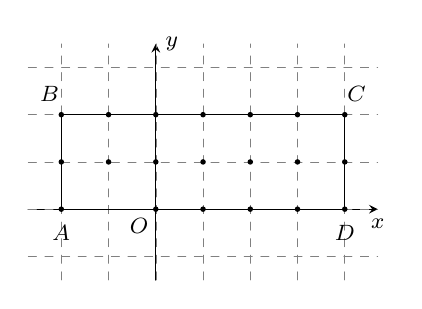
\begin{tikzpicture}[scale=1,font=\footnotesize,line join=round,line cap=round,>=stealth,x=0.6cm,y=0.6cm]
					\def  \xmin{-2.7};
					\def \xmax{4.7}; 
					 \def \ymin{-1.5};
					\def \ymax{3.5}; 
					\draw[->] (\xmin,0.)  -- (\xmax,0.) node[anchor=north] {$x$};
					\draw[->] (0.,\ymin) --  (0.,\ymax) node[anchor=west] {$y$};
					 \draw[step=1,gray,very thin,dashed] (\xmin,\ymin) grid (\xmax,\ymax);
					\clip (\xmin+0.1,\ymin+0.1) rectangle (\xmax-0.1,\ymax-0.1); 
					 \draw (-2,0) rectangle (4,2);
					\foreach \x/\y in {-2/1,-1/1,-1/2,0/1,0/2,1/0,1/1,1/2,2/0,2/1,2/2,3/0,3/1,3/2,4/1} \fill[black] (\x,\y) circle (1pt); 
					\foreach \x/\y/\l/\g in {0/0/O/225,-2/0/A/-90,-2/2/B/120,4/2/C/60,4/0/D/-90}{\fill[black] (\x,\y) circle (1pt)+(\g:0.5)  node{$\l$};}
				\end{tikzpicture}
		\end{center}
		Ta  có $\Omega=\{(x;y)\mid -2\leq x\leq 4;0\leq y\leq 2\}$, với $x,y\in\mathbb{Z}$.\\
		Do đó,  $x\in\{-2;-1;1;2;3;4\}$ và $y\in\{0;1;2\}$.\\
		Suy ra $n(\Omega)=7\cdot  3=21$ (mỗi điểm là một giao điểm trên hình).\\
		Vì $A$ \lq\lq $x;y$  đều chia hết cho $2$\rq\rq\ nên ta có $A=\{(x;y)\mid x\in\{-2;0;2;4\};y\in\{0;2\}\}$.\\
		Theo quy  tắc nhân ta có $n(A)=4\cdot 2=8$.
	} 
\end{ex}

% nguồn: MaHoaNH_TracNghiem_Lop10
\begin{ex}%[0D0C1-3]%[ma:37bd70a4]
	Một hội đồng quản trị gồm $10$ người, trong đó có $7$ nam và $3$ nữ. Cần lập ra một ban thường trực gồm chủ tịch, giám đốc, phó giám đốc và hai  thư ký. Mỗi người chỉ giữ một chức vụ. Số phần tử của biến cố \lq\lq lập được ban thường trực có ít nhất một nữ\rq\rq\ là
	 \choice
		 {$15\,120$}
		{\True $13\,860$} 
		 {$1\,260$}
		{$3\,528$} 
	\loigiai{Để lập một ban thường trực gồm chủ tịch, giám  đốc, phó giám đốc và hai thư ký (mỗi người chỉ giữ một chức vụ) sao cho ban thường trực có ít nhất một nữ ta làm bằng phương pháp phần bù.\\
		Gọi $A$ là  biến cố: \lq\lq Ban thường trực có ít nhất một nữ\rq\rq.\\
		Suy ra $\overline{A}$: \lq\lq Ban thường trực không  có nữ\rq\rq.\\
		Để lập một ban thường trực gồm chủ tịch,  giám đốc, phó giám đốc và hai thư ký (mỗi người chỉ giữ một chức vụ) ta làm như sau:\\
		Chọn $5$ người trong $10$ người để vào ban thường trực có $\mathrm{C}_{10}^5$ cách.\\ 
		Từ ban thường trực ta phân chia nhiệm vụ như sau: $5$ cách chọn chủ tịch; $4$ cách chọn giám đốc có $3$ cách chọn phó giám đốc hai người còn lại sẽ làm thư ký. Nên số cách để phân chia nhiệm vụ là $5\cdot 4\cdot 3=60$ cách.\\ 
		Theo quy tắc nhân  có $\mathrm{C}_{10}^5\cdot 60=15\,120$ cách lập một ban thường trực.\\
		Để lập một  ban thường trực trong đó không có nữ ta làm như sau:\\
		Chọn $5$ người trong $7$ nam để vào ban thường  trực có $\mathrm{C}_7^5$ cách.\\
		Từ ban thường trực ta phân  chia nhiệm vụ như sau: $5$ cách chọn chủ tịch; $4$ cách chọn giám đốc có $3$ cách chọn phó giám đốc hai người còn lại sẽ làm thư ký nên số cách để phân chia nhiệm vụ là $5\cdot 4\cdot 3=60$ cách.\\
		Theo quy tắc nhân có $n\left(\overline{A}\right)=\mathrm{C}_7^5\cdot  60=1\,260$ cách. \\
	Vậy số cách lập ban thường trực có ít nhất một nữ là  $n(A)=15\,120-1\,260=13\,860$.}
\end{ex}


%%%%%%%%%%%%%%%% ĐÚNG/SAI %%%%%%%%%%%%%%%%

% nguồn: MaHoaNH_DungSai_Lop10
\begin{ex}%[0D0N1-3]%[ma:7d04e421]
	Chọn các khẳng định đúng trong các khẳng định sau 
	\choiceTF 
		{\True ``Gieo $2$ con súc sắc'' có số phần tử không gian mẫu là $n\left( \Omega\right) =36$} 
		{``Gieo $2$ con súc sắc'' có  không gian mẫu là $ \Omega =36$}
		{\True ``Gieo  ba đồng xu phân biệt''thì số phần tử không gian mẫu của phép thử là $n\left( \Omega\right) =8$}
		{``Gieo ba  đồng xu phân biệt''thì số phần tử không gian mẫu của phép thử là $n\left( \Omega\right)=6$}
	 \loigiai{
		\begin{itemchoice}
			\itemch ``Gieo $2$ con súc sắc'' có số phần tử không gian mẫu là $n\left( \Omega\right) =36$ là khẳng  định đúng.
			\itemch ``Gieo $2$ con súc sắc'' có không gian mẫu là $ \Omega  =36$'' là sai vì $n\left( \Omega\right) =36$.
			\itemch ``Gieo ba đồng xu phân biệt''thì số phần tử không gian mẫu của phép  thử $n\left( \Omega\right) =8$ là khẳng định đúng.
			``Gieo ba đồng xu phân  biệt''thì số phần tử không gian mẫu của phép thử $n\left( \Omega\right)=6$ là sai vì $n\left( \Omega\right)=2^3=8$.
		\end{itemchoice}
	} 
\end{ex}

% nguồn: MaHoaNH_DungSai_Lop10
\begin{ex}%[0D0N1-3]%[ma:05b91d61]
	Gieo một  con súc sắc cân đối và đồng chất $2$ lần. Cho các biến cố sau
	\begin{itemize}
		\item  $A$: ``Tổng số chấm trong hai lần gieo chia hết cho $5$''
		\item $B$: ``Mặt $5$ chấm  xuất hiện ít nhất một lần''
		\item $C$: ``Tổng số chấm trong  hai lần gieo không bé hơn $10$''
		\item  $D$: ``Tổng số chấm trong hai lần gieo bằng $7$''
	\end{itemize}
	Hãy chọn tất cả các khẳng định  đúng?
	 \choiceTF
		{\True $n(A)=7$} 
		 {$n(B)=12$}
		{\True $n(C)=6$} 
		{$n(D)=7$} 
	 \loigiai{
		\begin{itemize}
			\item Không gian mẫu là $\Omega=\{(x;y):1 \le x; y \le 6\}$, trong đó $x$ là số chấm trong lần gieo thứ nhất và $y$ là số chấm trong lần gieo thứ hai $(x; y \in \mathbb{R^*})$. 
			\item Theo quy tắc nhân, suy ra số phần tử không gian mẫu  là $n(\Omega)=6 \cdot 6= 36$.
		\end{itemize}
		\begin{itemchoice}
			\itemch Gọi $A$ là biến cố  :\lq\lq Tổng số chấm trong hai lần gieo chia hết cho $5$\rq\rq.\\
			Liệt kê, ta có $C=\{(1;4);(4;1);(2;3);(3;2);(5;5);(4;6);(6;4)\} \Rightarrow  n(A)=7$.
			\itemch Gọi $B$ là biến cố :\lq\lq Mặt $5$ chấm xuất  hiện ít nhất một lần\rq\rq.\\
			 Ta có $B=\{(1;5);(2;5);(3;5);(4;5);(5;5);(6;5);(5;1);(5;2);(5;3);(5;4);(5;6)\} n(B)=11$.
			\itemch Gọi $C$ là biến cố :\lq\lq Tổng số chấm trong hai lần gieo không  bé hơn $10$\rq\rq.\\
			Liệt kê,  ta có $C=\{(4;6);(6;4);(5;5);(5;6);(6;5);(6;6)\} \Rightarrow n(C)=6$.
			\itemch Gọi $D$ là biến  cố :\lq\lq Tổng số chấm trong hai lần gieo bằng $7$\rq\rq.\\
			Liệt kê, ta có $D=\{(1;6);(6;1);(2;5);(5;2);(3;4);(4;3)\}  \Rightarrow n(D)=6$.
		\end{itemchoice}
	} 
\end{ex}

% nguồn: MaHoaNH_DungSai_Lop10
\begin{ex}%[0D0N1-3]%[0D0H1-3]%[0D0K1-3]%[ma:73818f64]
	 Cho các chữ số $0$, $ 2 $, $ 3 $, $ 6 $, $ 7 $.
	\choiceTF 
		{\True Chọn ngẫu nhiên một chữ số, xác xuất để được chữ số $0$ là  $\dfrac{1}{5}$}
		{Chọn ngẫu nhiên một chữ số, số khả năng  thuận lợi để được chữ số là hợp số là $1$}
		{\True Số các số có $2$ chữ số khác nhau chia hết cho $3$ lập được  từ các chữ số đã cho là $5$}
		{\True Có $18$ số có $3$ chữ số khác nhau lập được từ các chữ số đã cho chia  hết cho $4$}
	 \loigiai{
		\begin{itemize}
			\item 
			Số phần tử của  không gian mẫu là $5$.\\
			Số khả  năng thuận lợi để chọn được chữ số $0$ là $1$.\\
			Do  đó,
			xác suất để được chữ số $0$ là $\dfrac{1}{5}$. 
			\item 
			Trong $5$ chữ số đã cho có $2$ hợp số là số $0$ và  $6$.\\
			Do đó, số khả năng thuận lợi để được chữ số  là hợp số là $2$.
			\item Các số có hai chữ số khác nhau chia  hết cho $3$ lập được từ các chữ số đã cho là
			$$27,\  30,\ 36,\ 60,\, 63,\ 72.$$
			Vậy có $6$ số có hai  chữ số khác nhau chia hết cho $3$.
			\item Gọi $\overline{abc}$ là số có $3$  chữ số khác nhau chia hết cho $4$.\\
			Ta có $\overline{bc}$ chia hết cho $4$  nên $\overline{bc}\in \{20;32;36;60;72;76\}$.\\
			Do đó: $\overline{bc}$ có $6$ cách chọn và ứng với mỗi $\overline{bc}$ đã chọn thì $a$ có $3$  cách chọn.\\
			Vậy số các số có $3$ chữ số khác nhau lập được từ các chữ số đã  cho chia hết cho $4$ là $6\cdot 3=18$ (số).
		\end{itemize}
		\begin{itemchoice}
			 \itemch Đúng.
			\itemch  Sai.
			\itemch  Sai.
			\itemch  Đúng.
		\end{itemchoice}
	} 
\end{ex}

% nguồn: MaHoaNH_DungSai_Lop10
\begin{ex}%[0D0H1-3]%[ma:e71d7e76]
	Một nhóm có $6$ bạn nam và $5$ bạn nữ. Chọn ngẫu nhiên cùng một lúc ra $4$ bạn đi làm công  tác tình nguyện. Các mệnh đề sau đúng hay sai?
	\choiceTF 
		{Số phần tử của không gian mẫu là  $7920$}
		{\True Số kết quả thuận lợi của biến  cố: \lq\lq Trong $4$ bạn được chọn có $2$ bạn nam và $2$ bạn nữ\rq\rq\,bằng $150$}
		{Số kết quả thuận lợi của biến cố: \lq\lq Trong $4$ bạn được chọn  có ít nhất $2$ bạn nữ\rq\rq\,bằng $225$}
		{Số kết quả thuận lợi của biến cố: \lq\lq Trong $4$ bạn được chọn có nhiều nhất $2$ bạn nữ\rq\rq\,bằng $260$} 
	 \loigiai{
		\begin{itemchoice}
			\itemch  Sai. \\
			Chọn $4$ bạn trong  $6 + 5 = 11$ bạn không tính đến thứ là tổ hợp chập $4$ của $11$ phần tử. Vậy số phần tử của không gian mẫu là $\mathrm{C}_{11}^{4} = 330$.
			\itemch Đúng. \\ 
			Chọn $4$ bạn  được chọn có $2$ bạn nam và $2$ bạn nữ, số các chọn là $\mathrm{C}_{6}^{2}\cdot \mathrm{C}_{5}^{2} = 150$. Vậy có $150$ kết quả thuận lợi.
			\itemch Sai. 
			\begin{itemize}
				\item Trường $4$ bạn được chọn có $2$ bạn nam và $2$ bạn nữ.\\ 
				Số cách chọn là $\mathrm{C}_{6}^{2}\cdot \mathrm{C}_{5}^{2} = 150$ cách. 
				 \item Trường $4$ bạn được chọn có $1$ bạn nam và $3$ bạn nữ.\\
				Số cách chọn là $\mathrm{C}_{6}^{1}\cdot  \mathrm{C}_{5}^{3} = 60$ cách.
				\item  Trường $4$ bạn được là $4$ bạn nữ.\\
				 Số cách chọn là $\mathrm{C}_{5}^{4} = 5$ cách.
			\end{itemize}
			Theo quy tắc  cộng có $ 150 + 60 + 5 = 215$ cách. Vậy có $215$ kết quả thuận lợi.
			 \itemch Sai.
			\begin{itemize}
				\item Trường $4$ bạn được chọn có $2$ bạn  nam và $2$ bạn nữ.\\
				 Số cách chọn là $\mathrm{C}_{6}^{2}\cdot \mathrm{C}_{5}^{2} = 150$ cách.
				\item Trường $4$ bạn được chọn có $3$ bạn nam và  $1$ bạn nữ.\\
				 Số cách chọn là $\mathrm{C}_{6}^{3}\cdot \mathrm{C}_{5}^{1} = 100$ cách.
				 \item Trường $4$ bạn được là $4$ bạn nam.\\
				Số cách chọn là $\mathrm{C}_{6}^{4}  = 15$ cách.
			\end{itemize}
			Theo quy tắc cộng có $ 150 + 100 + 15 = 265$ cách. Vậy  có $265$ kết quả thuận lợi.
		\end{itemchoice}
	} 
\end{ex}

% nguồn: MaHoaNH_DungSai_Lop10
\begin{ex}%[0D0H1-3]%[ma:234c08a5]
	Gọi $S$ là tập hợp các số tự nhiên có ba chữ  số. Chọn ngẫu nhiên một số từ tập $S$. Các mệnh đề sau đúng hay sai?
	 \choiceTF
		 {$n\left(\Omega\right) = 1000$}
		{\True Gọi $A$ là biến cố: \lq\lq  Chọn được số tự nhiên có các chữ số đôi một khác nhau\rq\rq, khi đó $n\left(\overline{A}\right) = 648$}
		{\True Gọi $B$ là biến cố: \lq\lq Chọn được số tự nhiên chia hết cho $5$\rq\rq, khi đó $n\left(B\right) =  180$}
		{Gọi $C$ là biến cố: \lq\lq Chọn được  số tự nhiên chẵn\rq\rq, khi đó $n\left(C\right) = 500$}
	 \loigiai{
		\begin{itemchoice}
			\itemch Sai. \\ 
			Xét số tự nhiên có ba chữ số dạng $\overline{abc}$, với $a$, $b$, $c$ thuộc tập hợp $\left\{0; 1; 2; 3; 4; 5; 6; 7; 8; 9\right\}$ và $a  \ne 0$.\\
			Chọn chữ số $a$ có $9$  cách chọn.\\
			Chọn chữ số  $b$ có $10$ cách chọn.\\
			Chọn chữ  số $c$ có $10$ cách chọn.\\
			Theo quy tắc nhân ta có $9 \cdot 10  \cdot 10 = 900$. Vậy $n\left(\Omega\right) = 900$.
			 \itemch Đúng.\\
			Xét số tự nhiên có ba chữ số dạng $\overline{abc}$, với $a$, $b$, $c$ đôi một khác nhau và thuộc tập hợp $\left\{0; 1; 2; 3; 4; 5; 6; 7; 8; 9\right\}$, $a \ne  0$.\\
			Chọn chữ số $a$ có $9$ cách  chọn.\\
			Chọn chữ số $b$ có $9$ cách chọn trong các chữ số  còn lại sau khi chọn $a$.\\
			Chọn chữ số $c$ có $8$ cách  chọn trong các chữ số còn lại sau khi chọn $a$ và $b$.\\
			Theo  quy tắc nhân ta có $9 \cdot 8\cdot 8 = 648$. Vậy $n\left(A\right) = 648$.
			 \itemch Đúng. \\
			Xét số tự nhiên có ba chữ số dạng $\overline{abc}$, với $a$, $b$, $c$ thuộc tập hợp $\left\{0; 1; 2; 3; 4; 5; 6; 7; 8; 9\right\}$, $a \ne 0$, $c$ thuộc tập hợp $\left\{0; 5\right\}$.\\ 
			Chọn chữ số $c$ có $2$ cách  chọn.\\
			Chọn chữ số  $a$ có $9$ cách chọn.\\
			Chọn chữ số $b$ có  $8$ cách chọn.\\
			Theo quy tắc nhân ta có $2 \cdot 9\cdot 10 = 180$. Vậy $n\left(B\right) = 180$. 
			\itemch  Sai. \\
			Xét số tự nhiên có ba  chữ số dạng $\overline{abc}$, với $a$, $b$, $c$ thuộc tập hợp $\left\{0; 1; 2; 3; 4; 5; 6; 7; 8; 9\right\}$, $a \ne 0$, $c$ thuộc tập hợp $\left\{0; 2; 4; 6; 8\right\}$.\\
			Chọn chữ số $c$ có $5$ cách  chọn.\\
			Chọn chữ số $a$ có  $9$ cách chọn.\\
			Chọn chữ số  $b$ có $10$ cách chọn.\\
			Theo quy tắc nhân ta có $5 \cdot 9\cdot  10 = 450$. Vậy $n\left(B\right) = 450$.
		\end{itemchoice}
	 }
\end{ex}

% nguồn: MaHoaNH_DungSai_Lop10
\begin{ex}%[0D0H1-3]%[ma:360d94a3]
	Gieo đồng thời hai viên xúc xắc $6$ mặt cân đối  và đồng chất. Xét tính đúng sai của các khẳng định sau:
	\choiceTF 
		 {$n(\Omega)=12$}
		{\True Gọi $A$ là biến cố: \lq\lq Số chấm xuất  hiện trên mỗi viên xúc xắc là một số chẵn\rq\rq, khi đó $n(A)=9$}
		{\True  Gọi $B$ là biến cố: \lq\lq Số chấm xuất hiện trên mỗi viên xúc xắc là một số lẻ\rq\rq, khi đó $n(B)=9$}
		{Gọi $C$ là biến cố: \lq\lq Số chấm xuất hiện trên mỗi viên xúc xắc là  bằng nhau\rq\rq, khi đó $n(C)=1$}
	\loigiai{ 
		Ta lập được bảng mô tả không  gian mẫu như sau
		\begin{center}
			\begin{tikzpicture}
					\begin{scope}[xscale=1.8]
						 \path
						 (0,0) foreach \i[count=\k] in {$1$ chấm,$2$ chấm,$3$ chấm,$4$ chấm,$5$ chấm,$6$ chấm}{++(1,0) node (1\k){\i}}
						(0,-1) node {$1$ chấm} foreach \i[count=\k] in {$(1; 1)$,$(2; 1)$,$(3; 1)$,$(4; 1)$,$(5; 1)$,$(6; 1)$}{++(1,0)  node (2\k){\i}}
						(0,-2) node {$2$ chấm} foreach \i[count=\k] in {$(1; 2)$,$(2;  2)$,$(3; 2)$,$(4; 2)$,$(5; 2)$,$(6; 2)$}{++(1,0) node (3\k){\i}}
						(0,-3) node {$3$ chấm}  foreach \i[count=\k] in {$(1; 3)$,$(2; 3)$,$(3; 3)$,$(4; 3)$,$(5; 3)$,$(6; 3)$}{++(1,0) node (4\k){\i}}
						(0,-4) node {$4$ chấm} foreach \i[count=\k] in {$(1; 4)$,$(2; 4)$,$(3; 4)$,$(4; 4)$,$(5; 4)$,$(6; 4)$}{++(1,0)  node (5\k){\i}}
						(0,-5)  node {$5$ chấm} foreach \i[count=\k] in {$(1; 5)$,$(2; 5)$,$(3; 5)$,$(4; 5)$,$(5; 5)$,$(6; 5)$}{++(1,0) node (6\k){\i}}
						(0,-6) node {$6$ chấm}  foreach \i[count=\k] in {$(1; 6)$,$(2; 6)$,$(3; 6)$,$(4; 6)$,$(5; 6)$,$(6; 6)$}{++(1,0) node (7\k){\i}};
						\draw[shift={(-0.5,0.5)}] (0,0) grid  (7,-7)
						(0,0)--(1,-1) 
						 (0,-1) node[above right]{\tiny Viên 2}
						(1,0) node[below left]{\tiny  Viên 1};
					\end{scope}
				\end{tikzpicture}
		\end{center}
		\begin{itemchoice}
			\itemch Ta có  $n(\Omega)=12$.
			\itemch  Ta có $A=\{(2;2),(2;4),(2;6),(4;2),(4;4),(4;6),(6;2),(6;4),(6;6)\}$.\\
			 Vậy $n(A)=9$.
			 \itemch Ta có $B=\{(1;1),(3;1),(5;1),(1;3),(3;3),(5;3),(1;5),(3;5),(5;5)\}$.\\
			Vậy $n(B)=9$. 
			 \itemch Ta có $C=\{(1;1),(2;2),(3;3),(4;4),(5;5),(6;6)\}$.\\
			Vậy $n(C)=6$. 
		\end{itemchoice}
	} 
\end{ex}


%%%%%%%%%%%%%%%% TRẢ LỜI NGẮN %%%%%%%%%%%%%%%%

% nguồn: MaHoaNH_TraLoiNgan_Lop10
\begin{bt}%[0D0V1-3]%[ma:74cfada1]
	Một nhóm bạn có $4$ bạn gồm $2$ bạn nam Mạnh, Dũng và $2$ nữ là Hoa, Lan được xếp ngẫu nhiên trên một ghế dài. Kí hiệu MDHL là cách sắp xếp theo thứ tự: Mạnh, Dũng, Hoa, Lan. 
	Tính số  phần tử của biến cố $A$: \lq\lq Xếp nam và nữ ngồi xen kẽ nhau\rq\rq.
	 \shortans{8}
	 \loigiai{
		Biến cố $A$: \lq\lq Xếp nam và  nữ ngồi xen kẽ nhau\rq\rq.\\
		Đánh số ghế theo thứ tự $1$, $2$, $3$ , $4$. Xếp hai bạn nam ngồi xen kẻ ở các vị trí $(1; 3)$ hoặc $(2; 4)$. Sau đó xếp hai  bạn nữ vào hai vị trí còn lại.\\
		Hai bạn nam đổi chỗ nhau và hai bạn nữ đổi chỗ nhau. Do đó số cách xếp là $2\cdot 2!\cdot 2! = 8$. Vậy $n\left(A\right) =  8$.
	 }
\end{bt}

% nguồn: MaHoaNH_TraLoiNgan_Lop10
\begin{bt}%[0D0V1-3]%[ma:63c52107]
	Một hộp chứa $10$ quả bóng được đánh số từ $1$ đến $10$. Bình và An mỗi người lấy  ra ngẫu nhiên $1$ quả bóng từ hộp. Có bao nhiêu kết quả thuận lợi cho biến cố \lq\lq Tích hai số ghi trên hai quả bóng chia hết cho $3$\rq\rq.
	\shortans{48} 
	 \loigiai{
		Gọi biến cố $A$: \lq\lq Tích  hai số ghi trên hai quả bóng chia hết cho $3$\rq\rq.\\
		Biến cố đối $\overline{A}$: \lq\lq Tích hai số ghi trên hai quả  bóng không chia hết cho $3$\rq\rq.\\
		Số cách Bình và An mỗi  người lấy ra ngẫu nhiên $1$ quả bóng từ hộp $n\left(\Omega\right) = 10\cdot 9 = 90$.\\
		 Trong các số từ $1$ đến $10$ có $7$ số không chia hết cho $3$. Suy ra $n\left(\overline{A}\right) = 7 \cdot 6 = 42$.\\
		 Suy ra $n\left(A\right) = n\left(\Omega\right) - n\left(\overline{A}\right) = 90 - 42 = 48$.
	 }
\end{bt}

% nguồn: MaHoaNH_TraLoiNgan_Lop10
\begin{bt}%[0D0V1-3]%[ma:3d3e4fa4]
	Có $20$ tấm thẻ được đánh số từ $1$ đến $20$. Lấy ngẫu nhiên $3$ thẻ.Tính số phần tử của biến cố $A$: \lq\lq Có ít nhất một số ghi trên thẻ được chọn chia hết cho  $5$\rq\rq.
	 \shortans{580}
	 \loigiai{
		Biến cố $A$: \lq\lq Có ít nhất một số ghi trên thẻ được  chọn chia hết cho $5$\rq\rq.\\
		Biến cố đối  $\overline{A}$: \lq\lq Không có một số nào ghi trên thẻ được chọn chia hết cho $5$\rq\rq.\\
		Trong $20$ tấm thẻ thì có $4$ tấm thẻ là số chia  hết cho $5$ và $16$ tấm thẻ là số không chia hết cho $5$.\\
		Chọn $3$ thẻ trong  $20$ thẻ có $\mathrm{C}_{20}^{3}$ cách.\\
		Chọn $3$ thẻ có số ghi trên thẻ là  số không chia hết cho $5$ có $\mathrm{C}_{16}^{3}$ cách, nên $n\left(\overline{A}\right) = \mathrm{C}_{16}^{3}$.\\
		Suy ra chọn $5$ thẻ có ít nhất một số ghi trên thẻ được  chọn chia hết cho $5$ có\\ $\mathrm{C}_{20}^{3} - \mathrm{C}_{16}^{3}= 1580$. Vậy $n\left(A\right) = 580$.
	 }
\end{bt}

% nguồn: MaHoaNH_TraLoiNgan_Lop10
\begin{bt}%[0D0V1-3]%[ma:5587eb25]
	Cho tập $Q = \left\{1; 2; 3; 4; 5; 6\right\}$. Từ tập $Q$ có thể lập được bao nhiêu số tự nhiên có $3$ chữ số khác nhau. Tính số phần tử  của biến cố sao cho số được chọn nhỏ hơn $345$.
	\shortans{50} 
	\loigiai{ 
		Gọi  $A$ là biến cố: \lq\lq Số được chọn nhỏ hơn $345$\rq\rq.\\
		Số  tự nhiên có ba chữ số thuộc $A$ là $\overline{abc}$, với $a$, $b$, $c$ thuộc $Q = \left\{1; 2; 3; 4; 5; 6\right\}$ và đôi một khác nhau.
		\begin{itemize}
			 \item Trường hợp $a = 3$.\\
			 $+$ Nếu $b = 4$ thì $c \in \{1; 2\}$. Có $2$ số tự nhiên thỏa mãn.\\
			$+$ Nếu $b \in \{1; 2\}$ thì  $b$ có $2$ cách chọn và $c$ có $4$ cách chọn. Có $2 \cdot 4 = 8$ số tự nhiên thỏa mãn.\\
			Trường hợp  này có $2 + 8 = 10$ số thỏa mãn.
			\item Trường hợp $a \in \{1;  2\}$.\\
			Khi đó $a$ có $2$ cách chọn, $b$ có $5$  cách chọn và $c$ có $4$ cách chọn. Vậy có $2\cdot 5\cdot 4 = 40$ số tự nhiên thỏa mãn.
		\end{itemize}
		Theo quy tắc cộng ta có $ 10 + 40 = 50$ số  tự nhiên thỏa mãn.
		Do  đó $n\left(A\right) = 50$.
	} 
\end{bt}


%%%%%%%%%%%%%%%% TỰ LUẬN %%%%%%%%%%%%%%%%

% nguồn: MaHoaNH_TuLuan_Lop10
\begin{bt}%[0D0V1-3]%[ma:8dd7b618]
	Chọn ngẫu nhiên một  số nguyên lớn hơn $3$ và nhỏ hơn $99$. Gọi $B$ là biến cố \lq\lq Số được chọn chia hết cho $3$\rq\rq. Hãy tính số các kết quả thuận lợi cho $B$.
	\loigiai{ 
		Gọi $B$ là biến cố \lq\lq Số được chọn chia hết cho  $3$\rq\rq.\\
		Suy ra $B = \left\{3k\mid k\in  \mathbb{N}, 1 < k <33\right\}$.
		Do  đó $n\left(B\right) = 31$.
	 }
\end{bt}

% nguồn: MaHoaNH_TuLuan_Lop10
\begin{bt}%[0D0V1-3]%[ma:03d153c1]
	Có ba chiếc hộp, hộp thứ nhất chứa $6$ bi xanh được đánh số từ $1$ đến $6$, hộp thứ hai chứa $5$ bi đỏ được đánh số từ $1$ đến $5$, hộp thứ ba chứa $4$ bi vàng được đánh số từ $1$ đến $4$. Lấy ngẫu nhiên ba viên bi. Tính số phần tử của biến cố $A$: \lq\lq Ba bi được chọn vừa khác màu vừa khác  số\rq\rq.
	\loigiai{ 
		Biến cố $A$:  \lq\lq Ba bi được chọn vừa khác màu vừa khác số\rq\rq.\\
		Vì ba bi được chọn vừa khác màunên ta phải chọn mỗi hộp $1$ viên.\\ 
		\begin{itemize}
			\item Chọn từ hộp  thứ ba $1$ viên bi vàng có $4$ cách chọn.
			\item Chọn từ hộp thứ hai $1$ viên bi đỏ có số khác với viên bi đã chọn từ hộp ba có $4$ cách chọn. 
			\item Chọn từ hộp thứ nhất $1$ viên bi xanh có số khác với số của hai viên  đã chọn từ hộp một và hai có $4$ cách chọn.
		\end{itemize}
		 Vậy có $4^3 = 64$ cách chọn. Suy ra $n\left(A\right) = 64$.
	 }
\end{bt}
